\documentclass{article}

% if you need to pass options to natbib, use, e.g.:
%     \PassOptionsToPackage{numbers, compress}{natbib}
% before loading neurips_2021

% ready for submission
\usepackage[preprint]{neurips_2021}

% to compile a preprint version, e.g., for submission to arXiv, add add the
% [preprint] option:
%\usepackage[preprint]{neurips_2021}

% to compile a camera-ready version, add the [final] option, e.g.:
%\usepackage[final]{neurips_2021}

% to avoid loading the natbib package, add option nonatbib:
%    \usepackage[nonatbib]{neurips_2021}

\usepackage[utf8]{inputenc} % allow utf-8 input
\usepackage[T1]{fontenc}    % use 8-bit T1 fonts
\usepackage{hyperref}       % hyperlinks
\usepackage{url}            % simple URL typesetting
\usepackage{booktabs}       % professional-quality tables
\usepackage{amsfonts}       % blackboard math symbols
\usepackage{nicefrac}       % compact symbols for 1/2, etc.
\usepackage{microtype}      % microtypography
\usepackage{xcolor}         % colors
\usepackage{graphicx}

\title{A Small Attempt to Create Short Term Earthquake Forecasts}




\author{%
  Timothy Shinners\\
  Matrikelnummer 6116598\\
  \texttt{timothy.shinners@student.uni-tuebingen.de} \\
  Github Repo: $\textrm{https://github.com/TimothyShinners/earthquakes\_dataLit2022}$
}


\begin{document}

\maketitle

\begin{abstract}
  We investigate the possibility of using earthquake activity in one region to create short-term earthquake forecasts in another region. We found that earthquakes on the continent of Africa are significantly better at signalling imminent earthquakes in the Middle East than an independent Poisson process. After an earthquake in the Middle East, another Middle Eastern earthquake occurs within one week in 14$\%$ of cases. However, after an earthquake in Africa, an earthquake occurs within one week in the Middle East in 0.22$\%$ of cases.
\end{abstract}


\section{Introduction}

Earthquakes are a type of natural disaster that impose a serious threat to many communities around the world. The ability to accurately produce a short-term forecast of even a single earthquake has the potential to save thousands of lives [1]. Currently, the USGS "focuses its efforts on the long-term mitigation of earthquake hazards... rather than by trying to accomplish short-term predictions," [1]. In this paper, we investigate the possibility of creating short-term earthquake forecasts using seismic activity in other regions around the world. 

\section{Data}

For this project, we use the Worldwide Earthquake Database, which can be found on Kaggle [2]. It includes every known significant earthquake in history, with "significant" being defined as "one that meets at least one of the following criteria: caused deaths, caused moderate damage (approximately \$1 million or more), magnitude 7.5 or greater, Modified Mercalli Intensity (MMI) X or greater, or the earthquake generated a tsunami" [2]. The data provides information for each earthquake, such as its longitude and latitude, magnitude, and date. Each earthquake is sorted into a region, based on location. 

This data set suffers from selection bias. Human ability to detect earthquakes has increased rapidly in the past century, meaning that there are many significant but older earthquakes that went unrecorded, so they are not included in the data set. To avoid this bias, we only use earthquakes that occurred during or after the year 2000. It should be noted that earthquakes are deemed significant if they caused deaths or significant property damage. This means there is selection bias where weaker earthquakes are included if they occur in populous areas. One method to fix this issue would be to only use earthquakes of magnitude 7.5 or greater. However, there have only been 81 such quakes since 2000. In order to keep enough data, we opted to deliberately ignore this issue. 

Some of the regions in the data set rarely suffer from earthquakes. For our analysis, we decided to only use regions in which at least 20 earthquakes have occurred since 2000. This leaves us with 1119 earthquakes from 11 different regions shown in Figure \ref{map}.


\begin{figure}[h]
\centering
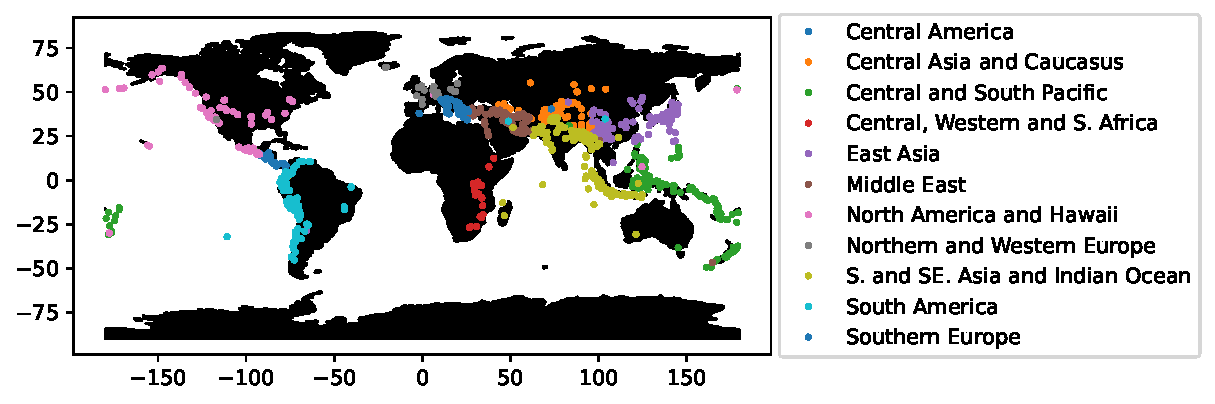
\includegraphics[scale=0.6]{new_quakes_world_map}
\caption{World map with all of the earthquakes used in our analysis, color coded by region.}
\label{map}
\end{figure}





\section{Do waiting times in different regions follow a Poisson process?}

The goal of this paper is to see if there exists a region whose earthquakes may signal an oncoming earthquake in another region. To this end, it would be very helpful if we could assume that the earthquakes in each region follow a Poisson process. Unfortunately this does not appear to be the case. If each region follows a Poisson process, then the number of earthquakes in a given interval of time should follow a Poisson distribution. For Poisson distributions, the mean and variance are equivalent. We counted the number of earthquakes per year in each different region. We then calculated the mean and variance of those counts. If the counts followed a Poisson process, we would expect to see that the mean of the counts are roughly equal to the variance of the counts. However, in Figure \ref{mean_v_var}, we see that, for the most part, the variances are larger than the means. This suggests that the earthquakes in most regions cannot be modelled by a Poisson process.

\begin{figure}
\centering
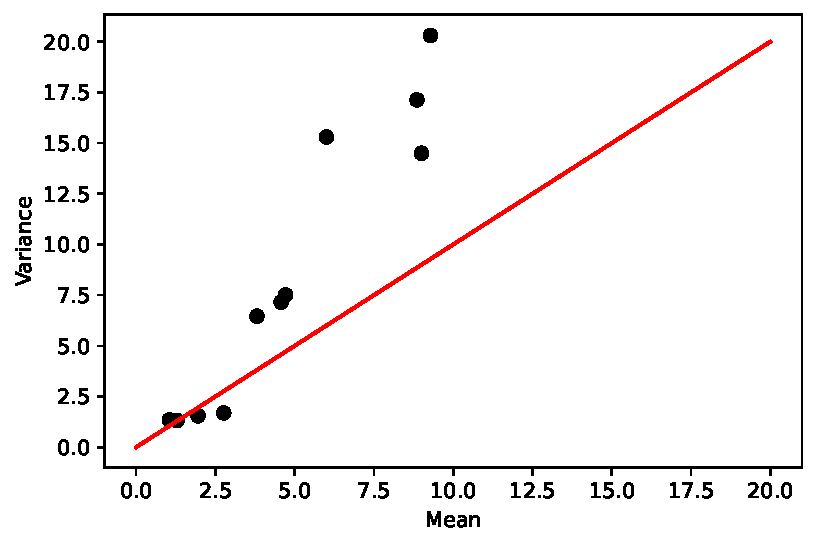
\includegraphics[scale=0.5]{mean_v_var.pdf}
\caption{Mean number of earthquakes per year vs. variance of earthquakes per year. Each point represents a different region. The line is what is expected if each region followed a Poisson process.}
\label{mean_v_var}
\end{figure}

\begin{figure}
\centering
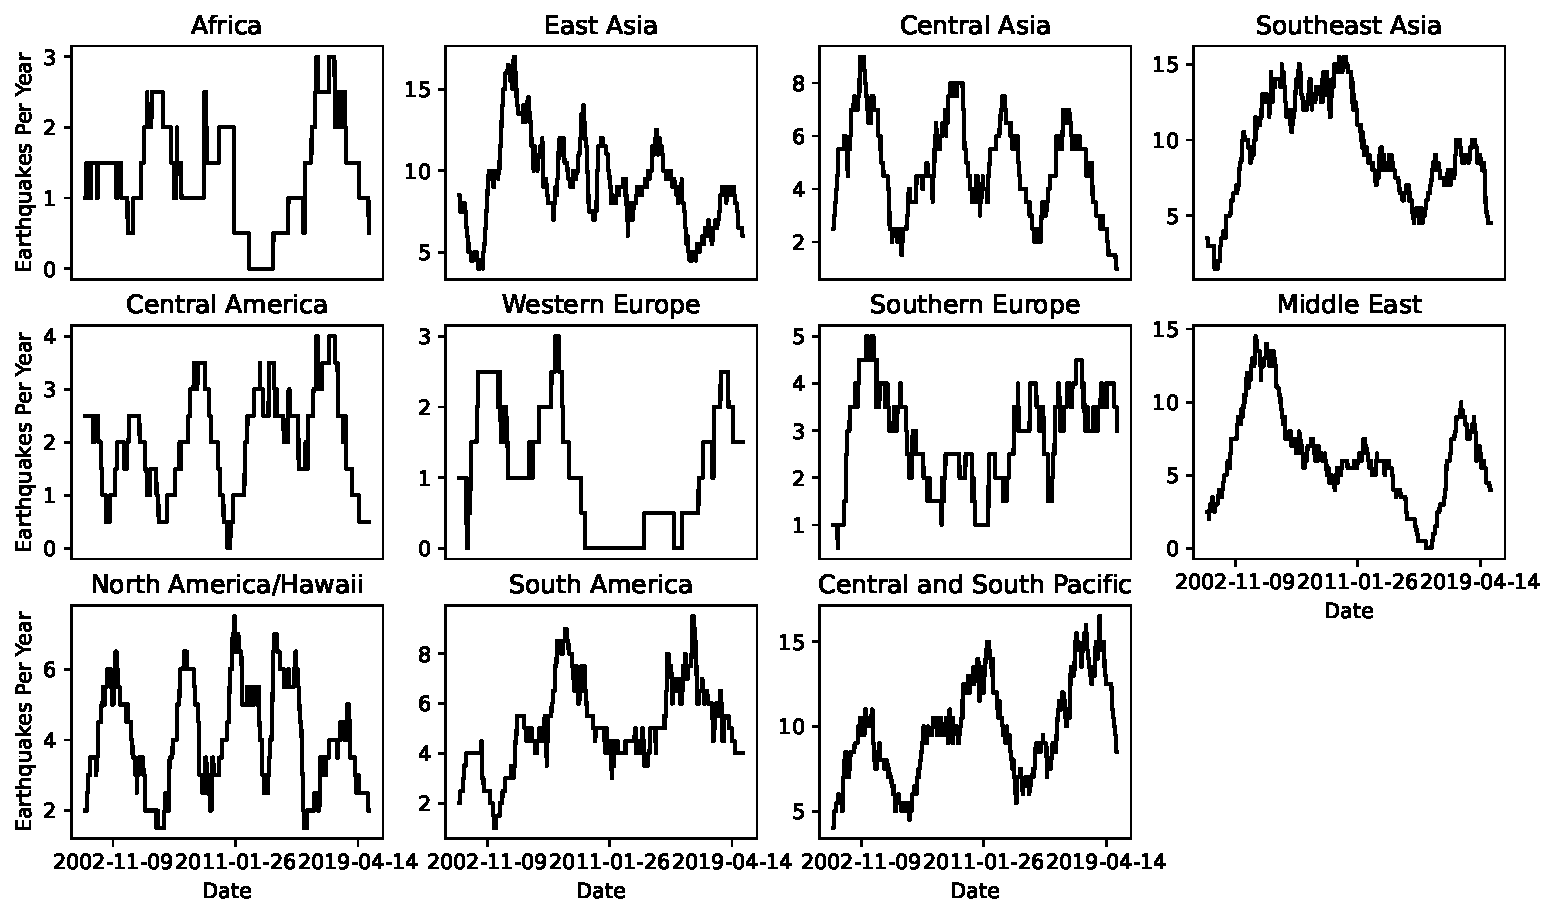
\includegraphics[scale=0.5]{localizedRates.pdf}
\caption{The y-axis shows the average number of earthquakes per year that occurred in a two year window centered around each date on the x-axis.}
\label{localizedRates}
\end{figure}

In order to further in the seismic patterns of each region, we calculated the mean number of earthquakes per year for a two year interval centered around each date since 2001. We did this for each region, and the results can be seen in Figure \ref{localizedRates}. This allows us to see that the localized rate of earthquake occurrences changes drastically over time, which further suggests that a Poisson process would be a poor model for our data. While we did not attempt it, this behavior could potentially be modelled by a non-homogeneous Poisson process. From here on out, we abandoned any attempts to assume the earthquakes of each region followed a particular statistical model.


\section{Can we use a specific region to influence short term earthquake forecasts in other regions?}


We still wanted to see if earthquakes in one region can signal an oncoming earthquake in another region. Let $i$ and $j$ be different regions. We started at the date of an earthquake in region $i$ and found the waiting time until the next earthquake in region $j$. We then used the information from Figure \ref{localizedRates} to calculate the expected waiting time in region $j$ for the given date. The true waiting time was then divided by the expected waiting time. This allowed us to control for the localized rate of earthquakes in the given time period. If this ratio was less than 1, then the earthquake in region $j$ happened unexpectedly soon after the quake in region $i$. We did this computation for each earthquake in region $i$, and then took the mean of the ratios and used it as a test statistic. Figure \ref{indicatorRatios} shows the value of this statistic for all pairs of regions. We used this information to determine which pairs may have the sort of relationship we were looking for. 



\begin{figure}
\centering
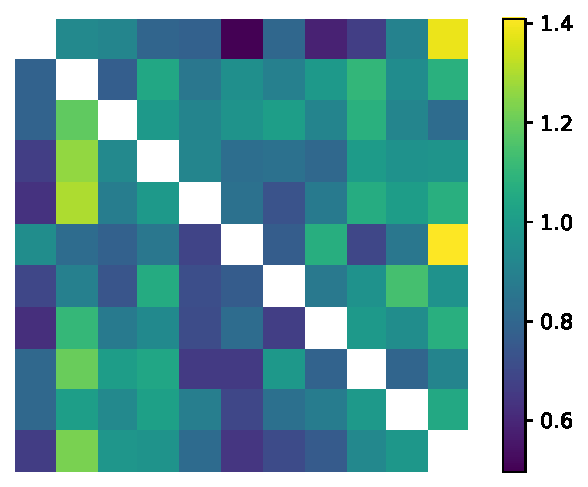
\includegraphics[scale=0.4]{indicatorRatios.pdf}
\caption{This plot shows the mean ratio between the actual waiting time for an earthquake in region x after an event in region y, and the expected waiting time in region y given the event date in region x. Smaller values suggests that an earthquake in region y may signal oncoming earthquakes in region x.}
\label{indicatorRatios}
\end{figure}



We wanted to test whether the values shown in Figure \ref{indicatorRatios} were significantly different than they would be if the earthquakes in the indicator region followed a Poisson process. Our test statistic, the mean of the ratios between waiting times and expected waiting times, comes from a completely unknown distribution, so in order to calculate p-values, we needed to create a bootstrap distribution. This was found to be computationally expensive, so we did not create a bootstrap distribution for every pair of regions. Instead, we created bootstrap distributions for only the pairs of regions with the five smallest test statistics. We figured that pairs of regions with the smallest test statistics were least likely to be randomly correlated. 

To create a bootstrap sample, we computed our test statistic, but using randomly sampled dates instead of the dates of earthquakes from the indicator region. We used 1000 samples to create a bootstrap distribution for each of the five pairs. From here, p-values were calculated as the proportion of bootstrap samples that were more extreme than the test statistic for each pair. The five pairs of regions, along with the calculated p-values, can be seen in Table \ref{p_value_table}. Three pairs are found to be significant at the 0.05 level. The two smallest values illuminate a probable relationship between Africa and the Middle East. The idea that these two regions share a relationship of this sort is reinforced by the fact that they are physically adjacent to each other.


\begin{table}
  \caption{Pairs of regions with smallest test statistics and calculated p-values}
  \label{p_value_table}
  \centering
  \begin{tabular}{llll}
    \toprule
    \cmidrule(r){1-2}
    Indicator Region     & Region  & Statistic   & P-value \\
    \midrule
    Central, Western and S. Africa & Northern and Western Europe & 0.496 & 0.087 \\ 
    Central, Western and S. Africa & Middle East & 0.583 & 0.018 \\
    Middle East & Central, Western and S. Africa & 0.618 & 0.046 \\
    Central America & Central, Western and S. Africa & 0.628 & 0.171 \\
    Central and South Pacific & Northern and Western Europe & 0.642 & 0.047 \\
    \bottomrule
  \end{tabular}
\end{table}

The fact that Africa and the Middle East appear to be good indicators for each other probably means that earthquakes in both regions happen in clusters. For now, we focus Africa's ability to signal imminent earthquakes in the Middle East. On average, after a significant earthquake in Africa, the waiting time for an earthquake is 0.58 of the localized expected waiting time in the Middle East. After an earthquake in the Middle East, another Middle Eastern earthquake occurs within one week in 14$\%$ of cases, but after an earthquake in Africa, an earthquake occurred in the Middle East within one week in 0.22$\%$ of cases.

\section{Discussion}

In our analysis, we uncovered a potential relationship between the regions of Africa and the Middle East. We found that African earthquakes are significantly better at signalling oncoming Middle Eastern earthquakes than an independent Poisson process would be. This suggests that there may be an increased risk of an earthquake in the Middle East in the days after an earthquake in Africa. 


The veracity of these results is debatable. We were unable to assume that the behavior of the individual regions followed a statistical model, which undermined our ability to test for dependencies between regions. Furthermore, we only used earthquakes from the past two decades, which is a mere snapshot in geologic time. We do not know how the different regions behave over longer time periods, and this extra information could drastically alter our results. The correlation in activity between Africa and the Middle East may have happened by chance, and it is conceivable that we would not see the same results with an observation period that lasts hundreds or thousands of years.

Even if our findings are true and correct, this information is probably not very useful. The estimated increase of risk in the Middle East after an earthquake in Africa is not drastic, and the Middle East covers a huge area. The statement, "there is a slightly elevated risk that there might be an earthquake somewhere in this massive area of land," is not long-term enough to influence the decisions of policymakers regarding earthquake preparations. It is also not specific or urgent enough to incite immediate earthquake preparations, like evacuations. 

Further analysis should attempt to divide the regions into smaller sub regions. If we were able to provide short term risk assessments for smaller areas of land, then our forecasts might become specific enough to be acted upon. Also, the magnitude of the earthquakes should be taken into account. It would be extremely useful to know if there are changes in worldwide seismic activity in the days before large earthquakes. An alternate method would have been to look at groups of earthquakes that are clustered into a small time period. Then, we could look into which regions tend to appear in clusters together. Potentially, we could say something like "regions a, b, and c tend to appear in clusters together, so if we see a quick succession of earthquakes in regions a and b, we should expect an increased risk in region c". This method might help to make our forecasts more specific with regards to the timing of an earthquake as well. 

\section*{References}



{
\small

[1] USGS, \ article, \ no date, \  https://www.usgs.gov/faqs/can-you-predict-earthquakes

[2] Kumar, Mohit, \ data set and description, \ 2020-06-08, \  https://www.kaggle.com/mohitkr05/global-significant-earthquake-database-from-2150bc
}

\end{document}
